\begin{table*}[ht]
    \centering
    \begin{tabular}{ccc|cc}
    \toprule
         & \multicolumn{2}{c}{AUC} & \multicolumn{2}{c}{$C_\text{max}$} \\
        $R$ & Random & Even & Random & Even\\
        \midrule
        $1$ & $0.893 \pm 0.022$ & $0.903 \pm 0.022$ & $91.43 \pm 1.60$ & $91.01 \pm 1.80$ \\ 
        \cmidrule{1-5}
        $2$ & $0.891 \pm 0.026$ & $0.890 \pm 0.025$ & $79.97 \pm 1.35$ & $73.46 \pm 1.86$ \\ 
        \cmidrule{1-5}
        $4$ & $0.869 \pm 0.022$ & $0.861 \pm 0.024$ & $61.40 \pm 1.77$ & $41.26 \pm 0.82$ \\ 
         \cmidrule{1-5}
        $8$ & $0.840 \pm 0.027$ & $0.834 \pm 0.029$ & $42.39 \pm 1.47$ & $21.51 \pm 0.51$ \\  
         \cmidrule{1-5}
        $16$ & $0.783 \pm 0.032$ & $0.754 \pm 0.032$ & $25.90 \pm 0.70$ & $10.90 \pm 0.23$ \\ 
         \cmidrule{1-5}
        $32$ & $0.682 \pm 0.022$ & $0.646 \pm 0.041$ & $13.54 \pm 0.42$ & $5.89 \pm 0.13$ \\ 
         \bottomrule
    \end{tabular}
    \caption{AUC and $C_\text{max}$ (mean and standard deviation) for \emph{Random} and \emph{Even} replacement position distribution.}
    \label{tab:uniform_vs_random_distr}
\end{table*}

Fig.~\ref{fig:auc_vs_r_main} shows how the AUC varies for increasing number of replacements $R$ made to the fuzzy trap sequences. We find that the AUC only drops slightly for smaller values of replacements $R$. For $R=4$, when $n_{\text{dup}}=10$ fuzzy trap sequences are injected, the mean AUC only drops from $0.90$ to $0.87$. Even at $R=32$, when we replace roughly one third of all tokens in the sequence, the mean AUC is $0.68$ and remains significantly higher than a single repetition $n_{\text{dup}}=1$ with a mean AUC of $0.59$. This demonstrates the mosaic memory in the target LLM, i.e. the overlapping fragments of multiple, slightly different sequences contribute to the memorization of the reference trap sequence.

\subsection{Replacement position distribution.} \label{section:spread_replacements}

We now aim to further reduce the chances of fuzzy trap sequences being removed by deduplication, and ensure that token replacements are evenly spread across the sequence. Above, we have uniformly at random sampled tokens to be replaced across fuzzy duplicates. Here, we instantiate the exact same setup, but we split the tokenized reference trap sequence using the MLM tokenizer: $T_{\text{MLM}}(X_{\text{ref}}) = \{t_1,\ldots,t_N\}$ in $R$ equally-sized chunks of size $\lceil\frac{N}{R}\rceil$. We then replace exactly one (selected uniformly at random) token for every chunk. Below we refer to this strategy as \emph{Even}, and to the previously used strategy as \emph{Random}.

We also compute the length of subsequences repeated exactly within clusters of fuzzy duplicates, simulating a sequence-level deduplication algorithm. We define $C_\text{max}$ as the maximum length (in tokens) of a substring shared by at least two fuzzy duplicate sequences within a cluster. We report the mean $C_\text{max}$ across 100 clusters used in our experiments.

Table~\ref{tab:uniform_vs_random_distr} shows that for smaller values of $R$ (up to $R=8$) the AUC for \textit{randomly} and \textit{evenly} distributed token replacements remains highly similar. For larger values of $R$ ($R \geq 16$), the impact of uniform spreading becomes more apparent, leading to a slightly lower AUC. At the same time, $C_\text{max}$ is significantly lower for the evenly distributed token replacements, with the impact more pronounced at higher values of $R$. This demonstrates how a reasonable number of token replacements ($R=4$ or $R=8$) would evade even the sequence-level deduplication with the most aggressive threshold (e.g. $50$ tokens), while retaining significant memorization.

\subsection{MIAs adapted to fuzzy trap sequences.} \label{section:adapted_mia}

So far we have used the unmodified \textit{Ratio} attack~\cite{carlini2021extracting} to infer whether the reference trap sequence has been seen by the target model. Specifically, we compute a single $\alpha(X_{\text{ref}}) = \alpha(X_1)$ for each trap sequence, and do not utilize our knowledge of the fuzzy counterparts $\{X_i \mid i=2 \ldots n_{\text{dup}}\}$. To evaluate whether this could further improve detectability, we now compute the membership score for each of the fuzzy trap sequences, i.e. $\{\alpha(X_i) \mid i=1 \ldots n_{\text{dup}}\}$, and aggregate the membership scores with aggregation function $\mathcal{A}(\cdot)$, i.e. $\alpha_{\mathcal{A}}(X_{\text{ref}}) = \mathcal{A}\left( \{\alpha(X_i) \mid i=1 \ldots n_{\text{dup}}\}\right)$. We then compute $\alpha_{\mathcal{A}}(X_{\text{ref}})$ for each reference trap sequence. We compute AUC on a balanced set of \emph{members} and \emph{non-members}, and so generate fuzzy trap sequences for all non-member sequences too. As aggregation function $\mathcal{A}$ we consider the mean, median, minimum and maximum. We report the MIA AUC for all aggregation functions, and for $R=\{2, 8, 32\}$ for models trained in the main experiment (Fig.~\ref{fig:auc_vs_r_main}). As a baseline, we also provide the previously used MIA based on the reference trap sequence $\alpha(X_{\text{ref}})$ alone.

 Table~\ref{tab:custom_MIA} shows that aggregating the membership score on all fuzzy trap sequences $\alpha_{\mathcal{A}}(X_{\text{ref}})$ does not provide substantial benefits compared to the baseline. We attribute this to the fact that all fuzzy trap sequences $X_i$ only differ from $X_{\text{ref}}$ by $R$ replacements, and therefore the target model loss computed on the reference trap sequence likely captures an aggregation across its fuzzy trap sequences already.

\begin{table*}[ht]
    \centering
    \begin{tabular}{cccc}
    \toprule
         & \multicolumn{3}{c}{AUC} \\
        Aggregation $\mathcal{A}$ & $R=2$ & $R=8$ & $R=32$ \\
        \midrule
        $\alpha(X_{\text{ref}})$ - no aggregation & $0.891 \pm 0.026$ & $0.840 \pm 0.027$ & $0.682 \pm 0.022$ \\ 
         \midrule
         \midrule
        Mean & $0.870 \pm 0.021$ & $0.828 \pm 0.029$ & $0.683 \pm 0.026$ \\ 
         \cmidrule{1-4}
        Median & $0.869 \pm 0.028$ & $0.824 \pm 0.030$ & $0.692 \pm 0.039$ \\  
         \cmidrule{1-4}
        Minimum & $0.881 \pm 0.021$ & $0.823 \pm 0.030$ & $0.624 \pm 0.040$  \\ 
         \cmidrule{1-4}
        Maximum & $0.879 \pm 0.030$ & $0.821 \pm 0.034$ & $0.679 \pm 0.041$  \\ 
         \bottomrule
    \end{tabular}
    \label{tab:custom_MIA}
    \caption{AUC (mean and standard deviation) for MIA methodologies adapted to fuzzy trap sequences.}
\end{table*}



\subsection{Ablation studies.} \label{section:ablations}

\textbf{Token replacement hyperparameters.} We here explore whether the semantic coherence of fuzzy trap sequences $X_i$ affect memorization. For this, we vary the value $k$ when sampling replacements from the top-$k$ tokens predicted by the MLM when a fixed number $R=8$ of replacements are made (see Sec.~\ref{sec:method_gen_fuzzy}). Recall that thus far we only considered $k=50$ and that for $k=|\mathcal{V}_{\text{MLM}}|$ -which is $50,000$ for RoBERTa~\cite{liu2019roberta}-, we effectively randomly sample a token from the entire MLM vocabulary $\mathcal{V}_{\text{MLM}}$. In addition to sampling uniformly from the top $k$ tokens, we also consider sampling directly from the full probability distribution predicted by the MLM (\textit{Sample directly}).

Fig.~\ref{fig:robustness}(a) shows that the AUC decreases as $k$ increases. We find $k$ and AUC to be strongly correlated with a Spearman coefficient of $-0.47$ and a p-value of \num{4e-11}, suggesting that semantic coherence is important for mosaic memorization. Further, Fig.~\ref{fig:robustness}(b) compares the AUC for $k=50$ and $k=|\mathcal{V}_{\text{MLM}}|$ for increasing values of $R$. For a smaller amount of replacements $R$, the AUC for $k=50$ and random token replacement remains very similar. For larger values of $R$ the mean estimations start to diverge, yet with no statistically significant difference.

\textbf{Impact of learning rate.} We here show, that the key outcome of our experiments - the \emph{relative} memorization of fuzzy duplicates compared to exact duplicates holds regardless of the \emph{absolute} level of memorization. At a fixed number of training steps we can control the baseline memorization with varying learning rate. So far in previous experiments, we have considered a fixed learning rate of $\num{3e-6}$. Fig.~\ref{fig:robustness} (b) shows how for increasing learning rate the AUC for fuzzy trap sequences remains consistently slightly lower than the upper bound ($n_{dup} = 10$), while remaining significantly higher than the lower bound ($n_{dup} = 1$). This suggests that fuzzy trap sequences are also memorized in lower and higher memorization regimes. 

\begin{figure*}[ht]
\centering
\subfigure{
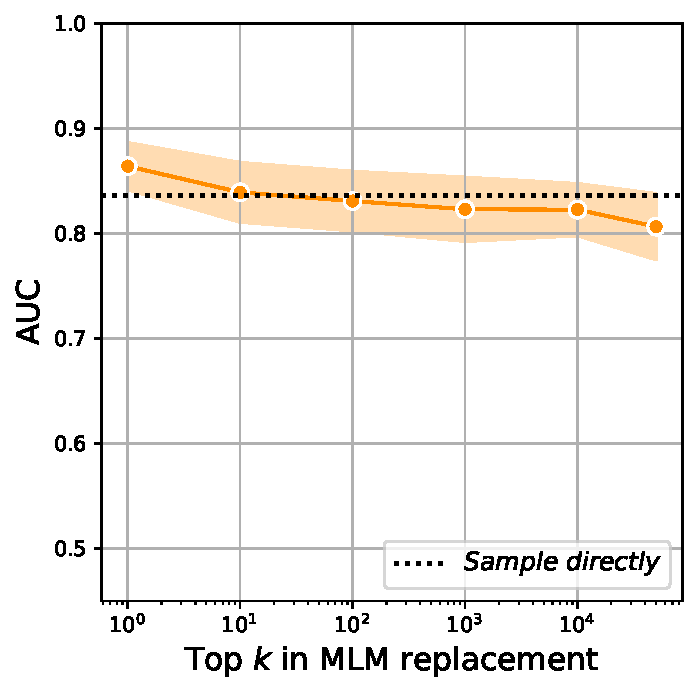
\includegraphics[width=0.3\linewidth]{figures/vary_k.pdf}
}
\subfigure{
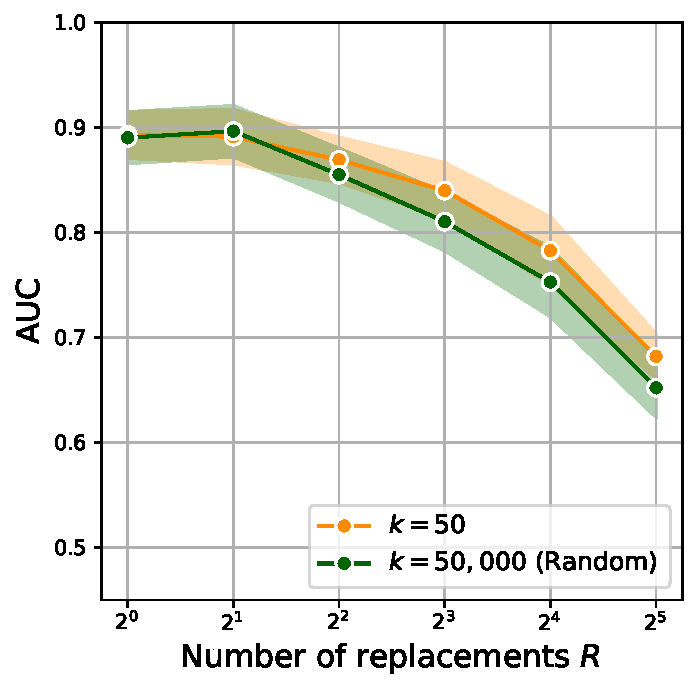
\includegraphics[width=0.3\linewidth]{figures/AUC_vs_R_both_strategies.pdf}
}
\subfigure{
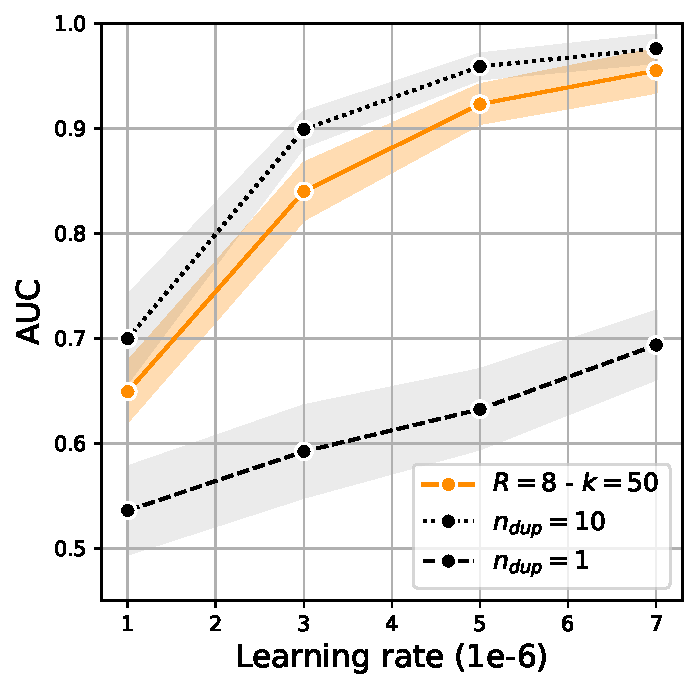
\includegraphics[width=0.3\linewidth]{figures/vary_lr.pdf}
}

    \caption{\textbf{Ablation.} MIA AUC (mean and standard deviation) for fuzzy trap sequences for (a) varying $k$ for $R=8$, (b) $k=50$ and $k=50,000$ across $R$ and (c) varying learning rate used in fine-tuning.} 
\label{fig:robustness}
\end{figure*} 
